%%%%%%%%%%%%%%%%%%%%%%%%%%%%%%%%%%%%%%%%%%%%%%%%%%%%%%%%%%%%%%%%%%%%%%%%%%%%%%%%
% Chapter 1: Introducción
%%%%%%%%%%%%%%%%%%%%%%%%%%%%%%%%%%%%%%%%%%%%%%%%%%%%%%%%%%%%%%%%%%%%%%%%%%%%%%%%

%+++++++++++++++++++++++++++++++++++++++++++++++++++++++++++++++++++++++++++++++

%+++++++++++++++++++++++++++++++++++++++++++++++++++++++++++++++++++++++++++++++


% \textcolor{red}{text}
%+++++++++++++++++++++++++++++++++++++++++++++++++++++++++++++++++++++++++++++++
\section{Antecedentes}
\label{1:sec:1}

Puntos clave: robots, sistemas guiados, camaras estereoscopicas, deteccion de
obstaculos

Las cámaras son uno de los sensores que pueden dar una información mas
rica del entorno para un robot. En este proyecto se plantea la utilización de
cámaras y de sistemas estereoscópicos de dos cámaras para la detección de
obstáculos y su posterior esquiva.


%+++++++++++++++++++++++++++++++++++++++++++++++++++++++++++++++++++++++++++++++
\section{Estado del arte}
\label{1:sec:2}


%+++++++++++++++++++++++++++++++++++++++++++++++++++++++++++++++++++++++++++++++
\section{Objetivo}
\label{1:sec:3}

El tema central de este proyecto es muy ambicioso, de este modo, es necesario
poder realizar una distinción entre el objetivo principal y los objetivos
específicos que lo rodean.

%--------------------------------------
\subsection{Objetivo general}

\textcolor{red}{¿Detección y esquiva o reconstrucción del mapa?}

El objetivo principal de este Trabajo de Fin de Grado es poder integrar el uso
de un sistema estereoscópico de dos cámaras en un robot, para la detección y
posteriormente esquiva de los obstáculos que se encuentren.

%--------------------------------------
\subsection{Objetivos específicos}

Los objetivos específicos que componen el proyecto son:
% \newline
\begin{itemize}
\item Uso de una cámara comercial de entretenimiento en un proyecto de
investigación.
\item Reconstrucción de un mapa tridimensional a partir de las imágenes
recogidas por las cámaras.
\item Integración de cámaras estereoscópicas junto a otros sistemas de detección
% \section{Sección Tres}
de obstáculos.
\end{itemize}


%+++++++++++++++++++++++++++++++++++++++++++++++++++++++++++++++++++++++++++++++
% \label{1:sec:3}
% \begin{itemize}
%   \item Item 1
%   \item Item 2
%   \item Item 3
% \end{itemize}
% Bla, bla, bla

%+++++++++++++++++++++++++++++++++++++++++++++++++++++++++++++++++++++++++++++++
% \section{Sección Cuatro}
%   \label{1:sec:4}
%
% Bla, bla, bla

%+++++++++++++++++++++++++++++++++++++++++++++++++++++++++++++++++++++++++++++++
% \begin{figure}[!th]
% \begin{center}
% \includegraphics[width=0.5\textwidth]{images/arbolbinario.eps}
% \caption{Ejemplo}
% \label{fig:ArbolBinario}
% \end{center}
% \end{figure}
%+++++++++++++++++++++++++++++++++++++++++++++++++++++++++++++++++++++++++++++++
